%%%%%%%%%%%%%%%%%%%%%%%%%%%%%%%%%%%%%%%%%
% Beamer Presentation
% LaTeX Template
% Version 1.0 (10/11/12)
%
% This template has been downloaded from:
% http://www.LaTeXTemplates.com
%
% License:
% CC BY-NC-SA 3.0 (http://creativecommons.org/licenses/by-nc-sa/3.0/)
%
%%%%%%%%%%%%%%%%%%%%%%%%%%%%%%%%%%%%%%%%%

%----------------------------------------------------------------------------------------
%	PACKAGES AND THEMES
%----------------------------------------------------------------------------------------

\documentclass{beamer}

\mode<presentation> {

% The Beamer class comes with a number of default slide themes
% which change the colors and layouts of slides. Below this is a list
% of all the themes, uncomment each in turn to see what they look like.

%\usetheme{default}
%\usetheme{AnnArbor}
%\usetheme{Antibes}
%\usetheme{Bergen}
%\usetheme{Berkeley}
%\usetheme{Berlin}
%\usetheme{Boadilla}
%\usetheme{CambridgeUS}
%\usetheme{Copenhagen}
%\usetheme{Darmstadt}
%\usetheme{Dresden}
%\usetheme{Frankfurt}
%\usetheme{Goettingen}
%\usetheme{Hannover}
%\usetheme{Ilmenau}
%\usetheme{JuanLesPins}
%\usetheme{Luebeck}
\usetheme{Madrid}
%\usetheme{Malmoe}
%\usetheme{Marburg}
%\usetheme{Montpellier}
%\usetheme{PaloAlto}
%\usetheme{Pittsburgh}
%\usetheme{Rochester}
%\usetheme{Singapore}
%\usetheme{Szeged}
%\usetheme{Warsaw}

% As well as themes, the Beamer class has a number of color themes
% for any slide theme. Uncomment each of these in turn to see how it
% changes the colors of your current slide theme.

%\usecolortheme{albatross}
%\usecolortheme{beaver}
%\usecolortheme{beetle}
%\usecolortheme{crane}
%\usecolortheme{dolphin}
%\usecolortheme{dove}
%\usecolortheme{fly}
%\usecolortheme{lily}
%\usecolortheme{orchid}
%\usecolortheme{rose}
%\usecolortheme{seagull}
%\usecolortheme{seahorse}
%\usecolortheme{whale}
%\usecolortheme{wolverine}

%\setbeamertemplate{footline} % To remove the footer line in all slides uncomment this line
%\setbeamertemplate{footline}[page number] % To replace the footer line in all slides with a simple slide count uncomment this line

%\setbeamertemplate{navigation symbols}{} % To remove the navigation symbols from the bottom of all slides uncomment this line
}
\usepackage[utf8]{inputenc}
% \usepackage[english]{babel}

\usepackage{graphicx} % Allows including images
\usepackage{booktabs} % Allows the use of \toprule, \midrule and \bottomrule in tables

%----------------------------------------------------------------------------------------
%	TITLE PAGE
%----------------------------------------------------------------------------------------

\title[The SprayList]{The SprayList:} % The short title appears at the bottom of every slide, the full title is only on the title page
\subtitle{A Scalable Relaxed Priority Queue}

\author[Autores]{Dan Alistarh\footnote{Microsoft Research}, Justin Kopinsky\footnote{MIT}, Jerry Li\footnote{MIT}, Nir Shavit\footnote{MIT and TAU} 
\newline 
\small{presented by} 
\newline \normalsize {Gabriel Aparicio, Luigy Machaca, Luis Cáceres} }  % Your name
\institute[UNSA] % Your institution as it will appear on the bottom of every slide, may be shorthand to save space
{
Universidad Nacional de San Agustín\\ % Your institution for the title page
\medskip
%\textit{-----------} % Your email address
}
\date{\today} % Date, can be changed to a custom date

\begin{document}

\begin{frame}
\titlepage % Print the title page as the first slide
\end{frame}

\begin{frame}
\frametitle{Overview} % Table of contents slide, comment this block out to remove it
\tableofcontents % Throughout your presentation, if you choose to use \section{} and \subsection{} commands, these will automatically be printed on this slide as an overview of your presentation
\end{frame}

%----------------------------------------------------------------------------------------
%	PRESENTATION SLIDES
%----------------------------------------------------------------------------------------

%------------------------------------------------
\section{Introduction}
%------------------------------------------------

\begin{frame}
\frametitle{Introduction}
High-performance concurrent priority queues are essential for applications
such as task scheduling and discrete event simulation.
Unfortunately, even the best performing implementations do not
scale past a number of threads in the single digits.\\

Starting from a nonblocking
SkipList, the main innovation behind our design is that
the DeleteMin operations avoid a sequential bottleneck by “spraying”
themselves onto the head of the SkipList list in a coordinated
fashion.

\end{frame}

\begin{frame}
\frametitle{Introduccion}
SkipLists are desirable because they allow priority queue insertions
and removals without the costly percolation up a heap or
the rebalancing of a search tree.\\
The SprayList provides probabilistic guarantees
on the relative priority of returned elements, and on the running
time of operations. At the same time, it shows fully scalable
throughput for up to 80 concurrent threads under high-contention
workloads.


\end{frame}

\begin{frame}
\frametitle{Image}
\begin{figure}
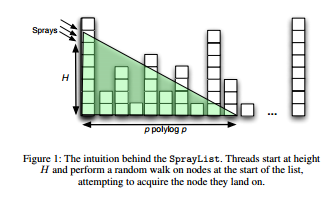
\includegraphics[width=0.8\linewidth]{SL1}
\end{figure}
\end{frame}


%------------------------------------------------
\section{The SprayList Algorithm}
%------------------------------------------------

\begin{frame}	
\frametitle{The SprayList Algorithm}
The data structure maintains an implementation of a set, defined by the bottom-level lock-free list. The SkipList is comprised of multiple levels,
each of which is a linked list. Every node is inserted deterministically
at the lowest level, and probabilistically at higher levels.\\
A key idea
in this design is that a node can be independently inserted at each
level. A node is $present$ if it has been inserted into the bottom list;
insertion at higher levels is useful to maintain logarithmic average
search time.

\end{frame}



\subsection{Spraying and Deletion}

\begin{frame}
\frametitle{Spraying and Deletion}

The goal of the Spray operation is to emulate a uniform choice
among the $O(plog3
p)$ highest-priority items. To perform a Spray,
a process starts at the front of the SkipList, and at some initial
height h. (See Figure 2 for an illustration.)

\begin{figure}
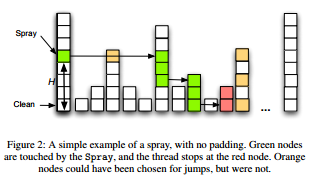
\includegraphics[width=0.5\linewidth]{SL2}
\end{figure}

\end{frame}



\begin{frame}
\frametitle{Spraying and Deletion}
Once on the bottom list, the process attempts to acquire the
current node. If the node is successfully acquired, the thread starts the standard SkipList removal procedure, marking the node as logically deleted.\\

\begin{itemize}
\item Spray Parameters.- In particular, notice that we can vary the starting height, the distribution for jump lengths at each level, and how many levels to descend between jumps.
\item Staring Height.-Each Spray starts at list level $H = log p + K$, for some constant $K^3$
\item Jump Length Distribution.- $L=M log^3 p$ where M is a constant value.
\item Level to Descend
\item Node Removal
\end{itemize}

\end{frame}




\subsection{Optimizations}

\begin{frame}
\frametitle{Optimizations}
\begin{itemize}
\item \textbf{Padding}.- A first practical observation is that, for small (constant)
values of D, the Spray procedure above is biased against elements at the front of the list.

\item \textbf{Cleaner}.- Before each new Spray, each thread flips a low probability
coin to decide whether it will become a cleaner thread.
\item \textbf{Adapting to Contention}.- In particular, a thread can estimate p, increasing its estimate if it detects higher than expected contention (in the form of
collisions) and decreasing its estimate if it detects low contention. 
\end{itemize}
\end{frame}



%------------------------------------------------
\section{Conclusions}
%------------------------------------------------

\begin{frame}
\frametitle{Conclusions}
\begin{itemize}
\item I have presented the PH-Tree as an approach for combined storage and indexing of multi-dimensional data.

\item In summary the combination of multi-dimensional indexing with space efficiency and good performance makes it a useful alternative for many applications.
\end{itemize}
\end{frame}

%------------------------------------------------
\section{References}
%------------------------------------------------

\begin{frame}
\frametitle{References}
\footnotesize{
\begin{thebibliography}{99} 
    \bibitem[Alistarh, 2015]{p1} Alistarh, Dan, et al.
    \newblock "The SprayList: A scalable relaxed priority 						queue." 
    \newblock \emph{ ACM SIGPLAN Notices 50.8 (2015): 11-20.}.
    \bibitem[K. Fraser, 2004]{p2}K. Fraser .
    \newblock "Practical lock-freedom." 
    \newblock \emph{ PhD thesis, PhD thesis, Cambridge
University Computer Laboratory, 2004}.
\end{thebibliography}
}
\end{frame}

%------------------------------------------------

\begin{frame}
\titlepage
\end{frame}

%----------------------------------------------------------------------------------------

\end{document}
